\documentclass[12pt,a4paper]{article}
\usepackage[utf8]{inputenc}
\usepackage[english,russian]{babel}
\usepackage{amssymb,amsfonts,amsmath,cite,enumerate,float,indentfirst}
\usepackage{graphicx}
\usepackage{geometry}
\usepackage{systeme}
\usepackage{hyperref}
\usepackage{url}
\usepackage[bottom]{footmisc}
\hypersetup{
	colorlinks,
	citecolor=black,
	filecolor=black,
	linkcolor=black,
	urlcolor=black
}
\geometry{left=2cm}
\geometry{right=1.5cm}
\geometry{top=2cm}
\geometry{bottom=2cm}

\begin{document}
	
\begin{titlepage}
	\begin{center}		
		\vfill	
		Санкт-Петербургский политехнический университет \\
		Петра Великого\\
		\vskip 1cm
		Институт прикладной математики и механики \\
		Кафедра «Прикладная математика»
		\vfill
		\textbf{Отчёт\\
			по лабораторной работе №4\\
			по дисциплине\\
			«Математическая статистика»\\}
		\vfill
	\end{center}
	\vfill
	\hfill
	\begin{minipage}{0.4\textwidth}
		Выполнил студент:\\
		Самутичев Евгений Романович\\
		группа: 3630102/70201\\
	\end{minipage}
	\vfill
	\hfill 
	\begin{minipage}{0.4\textwidth}
		Проверил:\\
		к.ф.-м.н., доцент\\
		Баженов Александр Николаевич\
	\end{minipage}
	\vfill
	\begin{center}
		Санкт-Петербург\\2020 г.
	\end{center}
\end{titlepage}

\tableofcontents
\listoffigures
\pagebreak

\section{Постановка задачи}
Для каждого из 5 распределений:

\begin{enumerate}
	\item Нормального $N(x, 0, 1)$
	\item Коши $C(x, 0, 1)$
	\item Лапласа $L(x, 0, \frac{1}{\sqrt{2}})$
	\item Пуассона $P(k, 10)$
	\item Равномерного $U(x, -\sqrt{3}, \sqrt{3})$	
\end{enumerate}

сгенерировать выборки размером 20, 60 и 100 элементов. Построить на них эмпирические функции распределения и ядерные оценки плотности/функции распределения на отрезке $[-4, 4]$ для непрерывных распределений и на отрезке $[6,14]$ для распределения Пуассона.
\pagebreak

\section{Теория}
\subsection{Эмпирическая функция распределения}
\textit{Эмпирической функцией распределения}, построенной по выборке $(x_1, ..., x_n)$ объема $n$ называется случайная функция $F_n^*: \mathbb{R} \times \Omega \to [0,1]$, которая имеет вид

\begin{equation}
	F_n^*(y) = \frac{1}{n}\sum_{i=1}^n{I(x_i < y)}
\end{equation}
где $I$ - индикатор события $x_i < y$\cite{chernova}

\subsection{Ядерная оценка плотности распределения}
Пусть $(x_1, ..., x_n)$ - выборка полученная по распределению с некоторой плотностью $f$, требуется оценить функцию $f$. \textit{Ядерным оценщиком плотности} называется\cite{kde}

\begin{equation}
	\hat{f}_h(x) = \frac{1}{nh}\sum_{i=1}^{n}{K\left(\frac{x-x_i}{h}\right)}
\end{equation}
где $K$ - т.н. \textit{ядро} (некоторая неотрицательная функция), $h>0$ - сглаживающий параметр, именуемый \textit{шириной полосы}.
\newline

Как правило используется нормальное (или гауссово) ядро, в силу его удобных математических свойств:
\begin{equation}
	K(x) = \frac{1}{\sqrt{2\pi}}e^{-\frac{x^2}{2}}
\end{equation}
\newline
\label{silverman}
В случае если используется гауссово ядро и оцениваемая плотность является гауссовой, оптимальный выбор для $h$ определяется т.н. \textit{правилом Сильвермана}\cite{kde}:
\begin{equation}
	h_n = \left(\frac{4s_n^5}{3n}\right)^{\frac{1}{5}}\approx 1.06s_n n^{-\frac{1}{5}}
\end{equation}
где $s_n$ - выборочное среднеквадратичное отклонение (корень из выборочной дисперсии)

\pagebreak

\section{Реализация}
\label{sec:impl}
Работа выполнена с использованием языка \textbf{Python} в интегрированной среде разработки \textbf{PyCharm}, были задействованы библиотеки:

\begin{itemize}
	\item \textbf{NumPy} - векторизация вычислений, работа с массивами данных
	\item \textbf{SciPy} - модуль \textbf{stats} для генерации данных по распределениям, вычисления ядерной оценки плотности
	\item \textbf{Matplotlib} - построение графиков
\end{itemize}

Исходный код работы приведен в приложении. 
\pagebreak

\section{Результаты}
\subsection{Эмпирические функции распределения}
\begin{figure}[h!]
	\centering
	\includegraphics[scale=0.8]{ecdf/normal.png}
	\caption{Нормальное распределение}
	\label{fig:image}
\end{figure}

\begin{figure}[h!]
	\centering
	\includegraphics[scale=0.8]{ecdf/cauchy.png}
	\caption{Распределение Коши}
	\label{fig:image}
\end{figure}
\pagebreak

\begin{figure}[h!]
	\centering
	\includegraphics[scale=0.8]{ecdf/laplace.png}
	\caption{Распределение Лапласа}
	\label{fig:image}
\end{figure}

\begin{figure}[h!]
	\centering
	\includegraphics[scale=0.8]{ecdf/poisson.png}
	\caption{Распределение Пуассона}
	\label{fig:image}
\end{figure}
\pagebreak

\begin{figure}[h!]
	\centering
	\includegraphics[scale=0.8]{ecdf/uniform.png}
	\caption{Равномерное распределение}
	\label{fig:image}
\end{figure}
\pagebreak

\subsection{Ядерные оценки плотности распределения}
\begin{figure}[h!]
	\centering
	\includegraphics[scale=0.8]{kde/normal.png}
	\caption{Нормальное распределение}
	\label{fig:image}
\end{figure}
\pagebreak

\begin{figure}[h!]
	\centering
	\includegraphics[scale=0.8]{kde/cauchy.png}
	\caption{Распределение Коши}
	\label{fig:image}
\end{figure}
\pagebreak

\begin{figure}[h!]
	\centering
	\includegraphics[scale=0.8]{kde/laplace.png}
	\caption{Распределение Лапласа}
	\label{fig:image}
\end{figure}
\pagebreak

\begin{figure}[h!]
	\centering
	\includegraphics[scale=0.8]{kde/poisson.png}
	\caption{Распределение Пуассона}
	\label{fig:image}
\end{figure}
\pagebreak

\begin{figure}[h!]
	\centering
	\includegraphics[scale=0.8]{kde/uniform.png}
	\caption{Равномерное распределение}
	\label{fig:image}
\end{figure}
\pagebreak

\section{Обсуждение}
\subsection{Эмпирическая функция распределения}
Существует \textbf{теорема} \cite{chernova}: \textit{Пусть $(x_1, ..., x_n)$ - выборка из распределения с некоторой функцией распределения $F$ и пусть $F_n^*$ - эмпирическая функция распределения построенная по этой выборке. Тогда $F_n^*(y) \overset{p}{\to} F(y), \forall y \in \mathbb{R}$} Полученные графики подтверждают данный теоретический факт, с ростом $n$ эмпирическая функцяи распределения все ближе к истинной. 

\subsection{Ядерная оценка плотности распределения}
Для нормального распределения наилучшие результаты показал выбор $h$ по правилу Сильвермана, что обосновано теоретически т.к. он оптимален в некотором смысле (см. \hyperref[silverman]{Теория}), как и для распределения Пуассона. Для распределения Лапласа хорошие результаты в приближении плотности распределения имеем как при $h_n$, так и при $0.5h_n$. Плотность равномерного распределения аппроксимируется неудачно т.к. оно далеко от гауссова, как и распределение Коши.
\pagebreak

\section{Приложения}
\noindent 1. Исходный код лабораторной {\url{https://github.com/zhenyatos/statlabs/tree/master/Lab4}}

\begin{thebibliography}{9} 
	\bibitem{chernova} Н. И. Чернова, \emph{Математическая статистика: Учеб. пособие}. Новосиб. гос. ун-т. Новосибирск, 2007. 148 стр.
	\bibitem{kde} Ядерная оценка плотности // Википедия. [2020—2020]. Дата обновления: 05.01.2020. URL: https://ru.wikipedia.org/?oldid=104368872 (дата обращения: 05.01.2020).
\end{thebibliography}

\end{document}
